\section{Indoor Positioning}\label{sec:indoor-positioning}

In order to determine which device the user points at and thereby intends to control, it is necessary to determine the locations of the devices in the system relative to the user.

The focus of this project is not to position devices and as such it was not the intention to spend time developing an entire solution for positioning devices indoors. Instead it was desired to find an existing product that could be used to facilitate indoor positioning.
The solution should be available in the early phases of the project in order to start building the system based on the solution for positioning.

Ideally users of this project should be able to control any device that fits within the concept of Internet of Things he owns, the price for any device needed to position each controllable device should be low. If a user owns several devices that can be controlled using gestures and an extra device is needed for each in order to preform the positioning, the price of such a device should be at a minimum.

It is assumed that users already own one or more devices that fit within the concept of Internet of Things and possibly are early adaptors of such technology, it is assumed they have some technological expertise. However, it easy to imagine that this project can be used in an office environment where employees of varying technological expertise work or in health care. Therefore users may have a varying degree of technological expertise and it should be easy to extend the solution with new controllable devices.

Naturally the accuracy of the solution used for positioning objects plays an important part. Figure \ref{fig:indoor-positioning:incorrect} shows the consequence of an incorrect location. If a lamp is estimated to be at another location that it is actually located, the user must point to an incorrect location in order to control the lamp.
Furthermore if the estimate is too wide, that is, the given area in which the lamp is located is very big, there is a greater risk that locations overlap. Overlapping locations causes a complexity as it is necessary to determine which device the user desires to control if he points at the overlap as visualized in figure \ref{fig:indoor-positioning:overlap}.

\begin{figure}[h]
\centering

\includegraphics[height=5cm]{images/incorrect-positioning-estimate.png}
\caption{Incorrect location estimate. The estimate is visualized as a striped circle.}
\label{fig:indoor-positioning:incorrect}
\end{figure}

\begin{figure}[h]
\centering
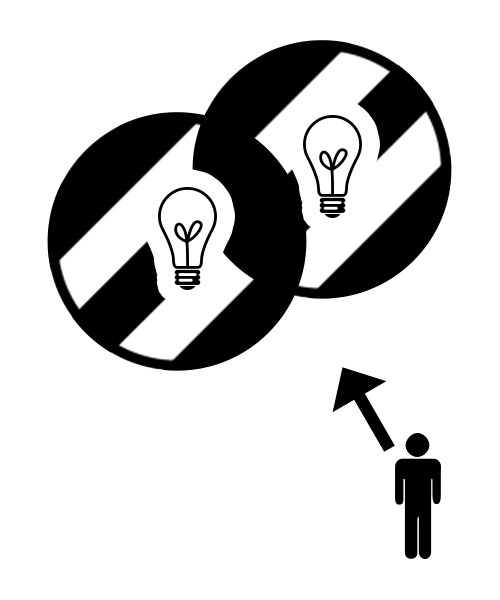
\includegraphics[height=5cm]{images/positioning-overlap.png}
\caption{Overlap of estimated positions. The estimates are visualized as a striped circle.}
\label{fig:indoor-positioning:overlap}
\end{figure}

Based on the above the following criterias for assessing potential solutions can be outlined.

\begin{itemize}
\item Availability
\item Price
\item Ease of use
\item Accuracy
\end{itemize}

Only solutions intended for indoor positioning was considered and thus GPS is not considered a potential solution. GPS is meant for outdoor positioning and a signal is not always aailable while indoors and even if it is, the accuracy of the estimated location is very low.

\begin{table}[h]
\centering
\caption{Assessement of potential solutions for indoor positioning. Please not that all prices are converted to U.S. dollars from their respective valuta. Prices include the minimum available hardware for positioning a device.}
\label{tbl:indoor-positioning}
\begin{tabularx}{\textwidth}{XXXXX}
\textbf{Product} & \textbf{Availability} & \textbf{Price} & \textbf{Ease of use} & \textbf{Accuracy} \\

Estimote Beacons and Stickers \cite{estimote}
& Beacons and Stickers are shipping. SDKs available.
& \$99 for beacons. \$99 for 10 stickers, one per device to be positioned.
& Initial installation of beacons. Attach each sticker to device.
& Unknown. Desired to be less than five meters. \todo[author=Simon]{Update after conducting tests.} \\

Pozyx \cite{pozyx}
& Available for preorder.
& \$368 for anchors. \$123 for each device to be positioned, plus supported Arduino.
& Initial installation of anchors. One tag for each device, plus supported Arduino. Not meant for mounting.
& Claimed to be 10 cm. Untested.

\end{tabularx}
\end{table}

\subsection{Methods of indoor positioning}
To locate devices and users inside buildings, various approaches were considered.

\begin{itemize}
\item Trilateration using signal strength (Eg. Wi-Fi or Bluetooth)
\item Fingerprinting of signal strength
\item Line of sight (Eg. Light)
\item Directional signals (Eg. Bluetooth)
\end{itemize}

\subsection*{Trilateration}
One way of getting the position of a user is to use the signal strength of a set of transmitters, eg. Wi-Fi access points. This requires that the position of each transmitter used is known so the position of the user relative to the transmitters can be determined.

If only one transmitter is used, then it is impossible to determine where the user is based on the distance alone. The only thing known is that the user is somewhere on the circumference of a circle centered around the transmitter with a radius equal to the distance between the user and the transmitter.
If two transmitters are used then there are two possible locations where the user may be, and that is where two circles centered on each transmitter respectively intersect.
When a third transmitter is introduced then there is only one point where the user can be.

However there are some uncertainties associated with this method because signal strength may vary in if the receiver remains stationary. This means that the distance between a user and a set of transmitters cannot be determined accurately based on signal strength alone.

\subsection*{Fingerprinting of Signal Strength}
Another method is to collect a dataset of signal strength values with an associated position submitted by person who noted the location where the signal strength was measured. When a sufficient\todo{Determine what constitutes sufficient in this case or reword.} amount of data has been acquired a user can get an estimated position by measuring signal strength and comparing it to the ones in the dataset.

\subsection*{Line of Sight}
Instead of trying to determine where users and devices are located, the user can send a light towards a receiver near a device. If the receiver is hit by the light then the device is selected. This approach requires an unobstructed path between the user and the devices as anything standing in between may block the light.

\subsection*{Directional Signals}
To combat things blocking a light, the user can send a directional signal that can penetrate some materials. By default Bluetooth signals are omnidirectional, meaning they are sent out in every direction around a transmitter. One way to solve this would be to build a casing around the transmitter blocking the signal in most directions leaving only a small spot open. Another would be to create a custom transmitter.

%%% Local Variables:
%%% mode: latex
%%% TeX-master: "../../master"
%%% End:
